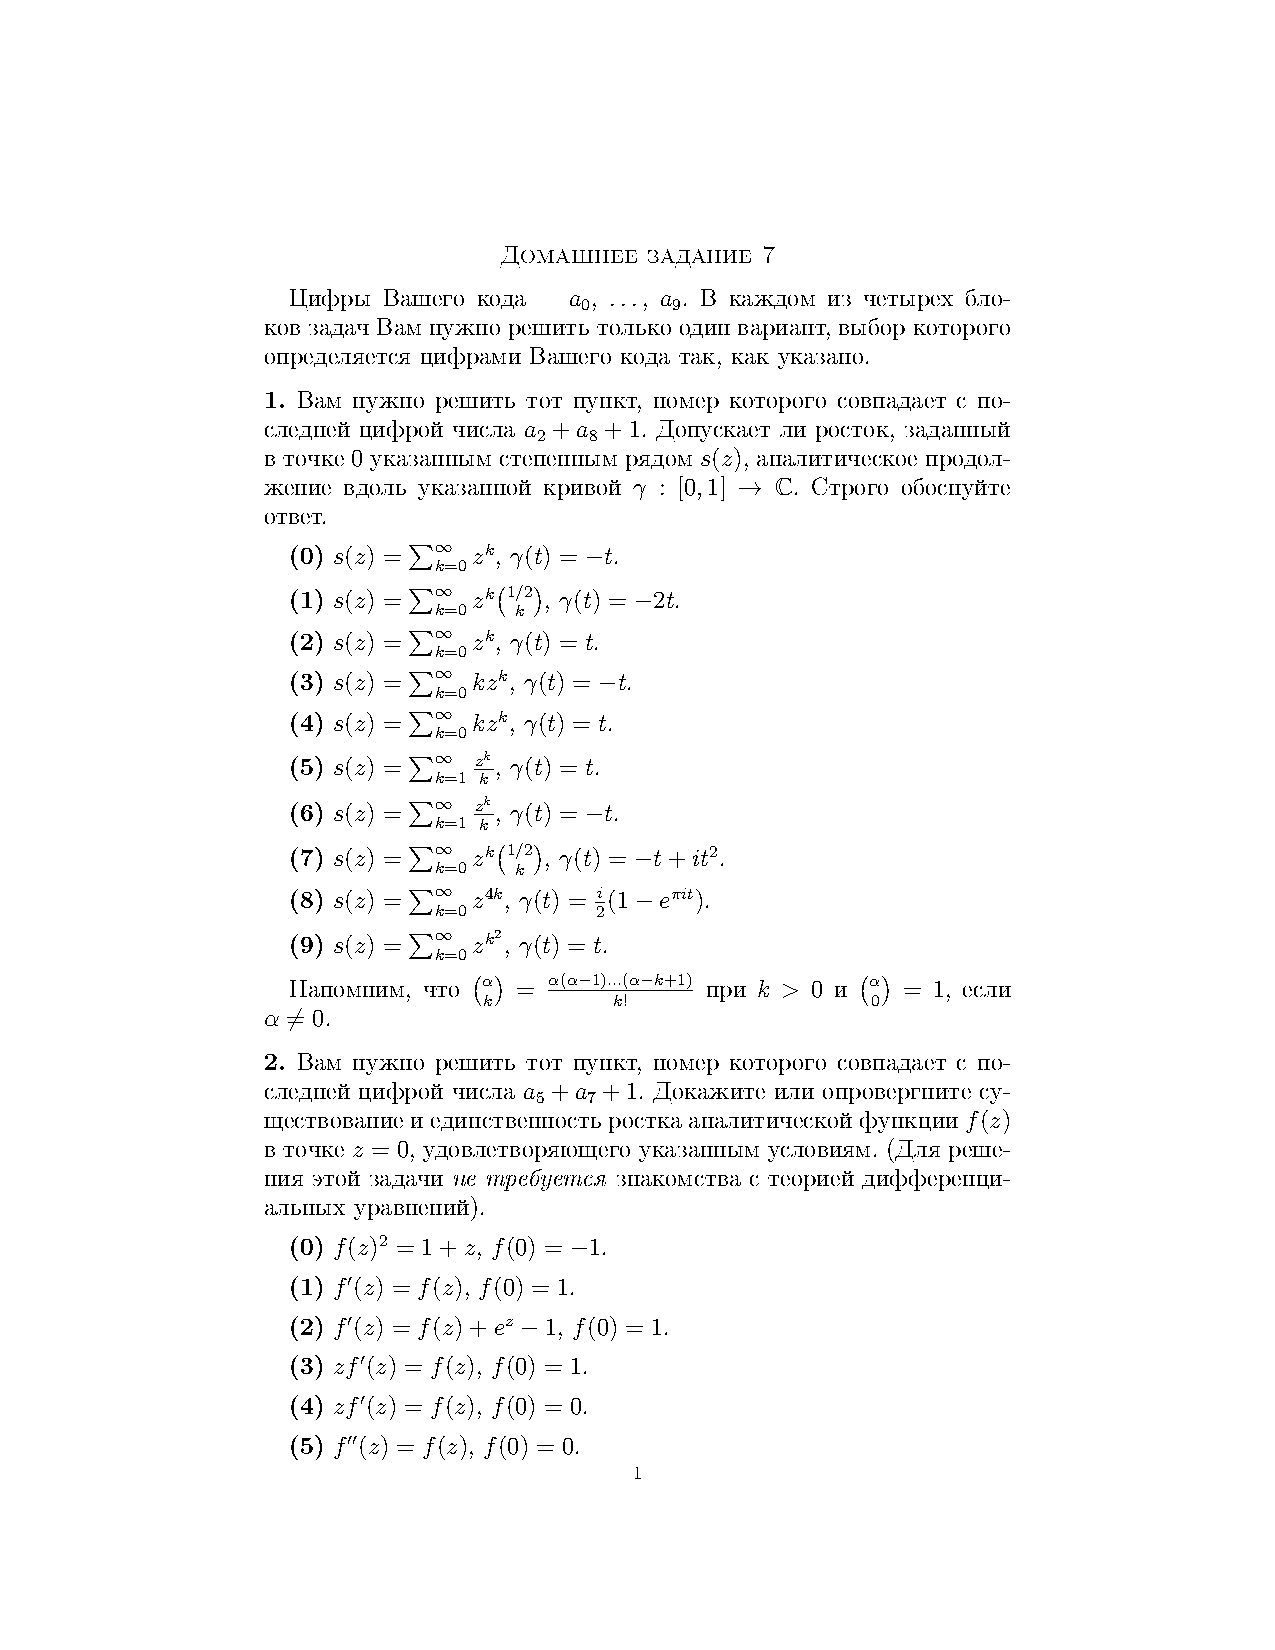
\includepdf[scale=1,pages=1-3]{Tasks/hw7}
\newpage
\section*{Решения}
\subsection*{Задача 1}
	Необходимо решить задачу $a_2 + a_8 + 1 = 8 + 8 + 1 = 7 \mod 10$
	\begin{gather*}
		s(z) = \sum\limits_{k = 0}^{\infty} z^k {{\frac{1}{2}}\choose{k}},\ \gamma(t) = -t + it^2
	\end{gather*}
	Радиус сходимости ряда 
	\begin{gather*}
		R = \lim\limits_{k \to \infty} \left|\frac{{{\frac{1}{2}}\choose{k}}}{{{\frac{1}{2}}\choose{k+1}}}\right| = 1
	\end{gather*}
	Заметим также что
	\begin{gather*}
		\sum\limits_{k = 0}^{\infty} z^k {{\frac{1}{2}}\choose{k}} = \sqrt{z+1}\\
		\gamma(0) = 0,\ \gamma(1) = i-1
	\end{gather*}
	Рассмотрим диск $D_1$ с центром в $0$ и радиусом $\frac{1}{\sqrt{2}}$, в нем $\sum\limits_{k = 0}^{\infty} z^k {{\frac{1}{2}}\choose{k}}$ сходится и $s: D_1 \to C$, теперь рассмотрим диск $D_2$ с центром в $(-1,1)$ и радиусом $\frac{3}{4}$ и $h: D_2 \to C$, так мы покрыли $\gamma$ двумя дисками, на пересечении $s,h$ совпадают, так как в этой области оба ряда сходятся к одной и той же функции $\sqrt{1+z}$. Росток допускает аналитическое продолжение вдоль $\gamma$ и $\sqrt{1+z}$ -- результат аналитического продолжения вдоль $\gamma$.
\vskip 0.4in

\subsection*{Задача 2}
	Необходимо решить задачу $a_5 + a_7 + 1 = 6 + 3 + 1 = 0 \mod 10$
	\begin{gather*}
		f(z)^2 = 1 + z,\ f(0) = -1
	\end{gather*}
	Пусть росток существует, тогда он имеет вид $f(z) = \sum\limits_{n = 0}^{\infty} a_n z^n$
	\begin{gather*}
		f(0) = -1,\ a_0 = -1\\
		f(z)^2
		= \left(\sum\limits_{n = 0}^{\infty} a_n z^n\right)^2
		= (a_0 + a_1 z + a_2 z^2 + \ldots)^2
		= a_0^2 + 2a_0 a_1 z + (a_1^2 + 2a_0 a_2)z^2 + \ldots
		= 1 + z\\
		2a_0a_1 = 2 \cdot (-1) \cdot a_1 = 1,\ a_1 = -\frac{1}{2}\\
		a_1^2 + 2a_0a_2 = \frac{1}{4} - 2a_2 = 0,\ a_2 = \frac{1}{8}\\
		2a_0a_3 + 2a_1a_2 = -2a_3 - \frac{1}{16} = 0,\ a_3 = -\frac{1}{32}\\
		a_n = \frac{(-1)^n}{2^{2n-1}}
	\end{gather*}
	А следовательно росток один


\vskip 0.4in

\subsection*{Задача 3}
	Необходимо решить задачу $a_2 + a_6 + 1 = 8 + 9 + 1 = 8 \mod 10$
	\begin{gather*}
		w^2 = z^2,\ w(1) = -1,\ \gamma(t) = e^{2\pi i t}
	\end{gather*}
	Заметим, что $\gamma(0) = e^{2 \pi i * 0} = e^{0} = 1, \gamma(1) = e^{2 \pi i * 1} = e^{2 \pi i} = (-1)^2 = 1$, тогда
	\begin{gather*}
		\omega^2 = z^2 \Rightarrow \omega = z \vee \omega = -z\\
		\omega(\gamma(0)) = -1
	\end{gather*}
	Далее нам нужно посмотреть, обходит ли график особые точки
	Если $\omega = z$, то график не обходит особые точки, если $\omega = -z$ то $\omega(z) = -1 \Leftrightarrow z = 1$ и $\omega(\gamma(1)) = \omega(1) = -1$. 
\vskip 0.4in

\subsection*{Задача 4}
	Необходимо решить задачу $a_0 + a_7 + 1 = 1 + 3 + 1 = 5 \mod 10$
	\begin{gather*}
		f(z) = \log(z),\ a = 1 + i,\ \Im(f(a)) \in \left[0,2\pi\right)
	\end{gather*}
	Заметим что на открытом шаре $B(z_0, |z_0|)$ мы можем определить логарифм как $f(z) = \log(z_0) + \int_{z_0}^{z} \frac{dz}{z}$, где контур $z_0-z$ содержится целиком в $B(z_0, |z_0|)$. Радиус сходимости не может быть больше $|z_0|$, так как $\log(z)$ не аналитическая в любой окрестности $z = 0$, а также по интегральной формуле Коши
	\begin{gather*}
		\frac{d^n}{dz^n} \log(z_0) = \frac{n!}{2\pi i} \int_{\gamma_{z_0, r}} \frac{\log(\omega) d \omega}{(\omega - z_0)^{n+1}}\\
		\gamma_{z_0, r}(t) = z_0 + re^{it},\ t \in [0, 2\pi]\\
		\omega \in \gamma_{z_0, r} \frac{|z_0| - r}{|z_0|} \leqslant \frac{|z_0| + r}{|z_0|}
	\end{gather*}
	Тогда
	\begin{gather*}
		|\log(\omega)| \leqslant \left(\frac{|z_0|^2}{|z_0|-r}\right)
	\end{gather*}
	Откуда
	\begin{gather*}
		\lim\limits_{n \to \infty}\sup \left|\frac{1}{n!} \frac{d^n}{dz^n} \log(z_0)\right|^{\frac{1}{n}}
		\leqslant \lim\limits_{n \to \infty}\sup \left|\frac{1}{r^{n+1}} \log \left(\frac{|z_0^2|}{|z_0|-r}\right)\right|^{\frac{1}{n}}
		= \frac{1}{r}
	\end{gather*}
	Радиус сходимости хотя бы $r$ для любого $r < |z_0|$, а следовательно он не менбше и равен $|z_0|$, то есть в нашем случае $|1 + i| = \sqrt{2}$

\vskip 0.4in
